\chapter{نمودارهای فعالیت}
برای هرکدام از موارد کاربرد، یک نمودار فعالیت رسم شده است که نام آن با نام مورد کاربرد رسم شده یکسان است.
\section{اضافه کردن پروژه}
\begin{figure}[H]
	\centering
	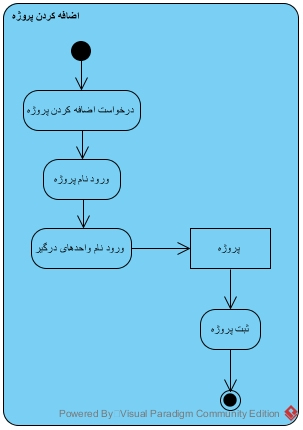
\includegraphics[scale=0.8]{img/activity/addproject}
	\caption{اضافه کردن پروژه}
\end{figure}

\section{اضافه کردن سیستم به پروژه}
\begin{figure}[H]
	\centering
	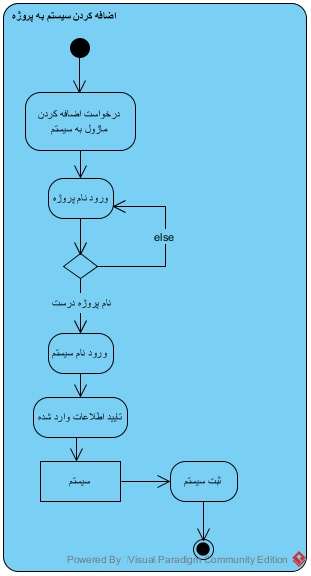
\includegraphics[scale=0.8]{img/activity/addsys}
	\caption{اضافه کردن سیستم به پروژه}
\end{figure}

\section{اضافه کردن ماژول به سیستم}
\begin{figure}[H]
	\centering
	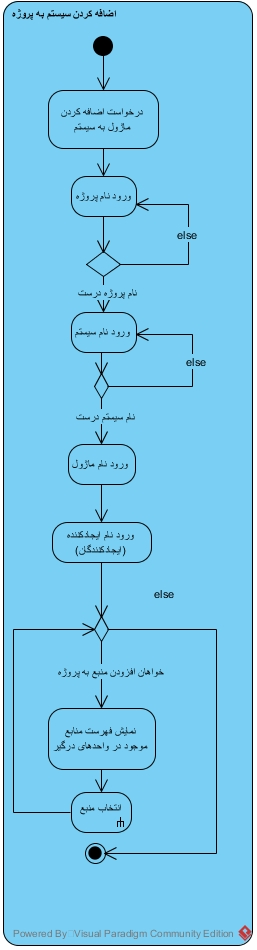
\includegraphics[scale=0.8]{img/activity/addmodule}
	\caption{اضافه کردن ماژول به سیستم}
\end{figure}

\section{اضافه کردن منبع به واحد سازمان}
\begin{figure}[H]
	\centering
	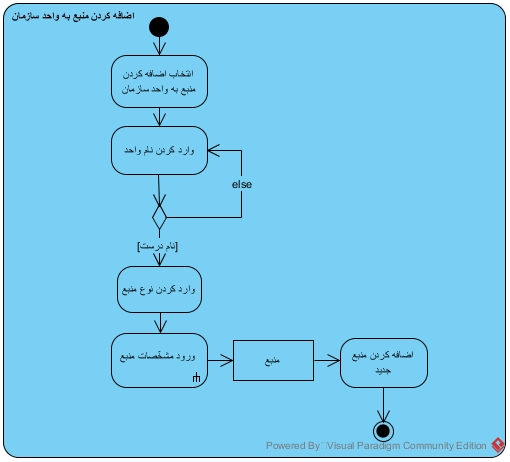
\includegraphics[scale=0.8]{img/activity/addresunit}
	\caption{اضافه کردن منبع به واحد سازمان}
\end{figure}

\section{افزودن واحد به سازمان}
\begin{figure}[H]
	\centering
	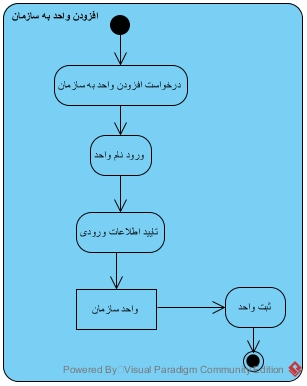
\includegraphics[scale=0.8]{img/activity/addunit}
	\caption{افزودن واحد به سازمان}
\end{figure}


\section{انتخاب منبع}
\begin{figure}[H]
	\centering
	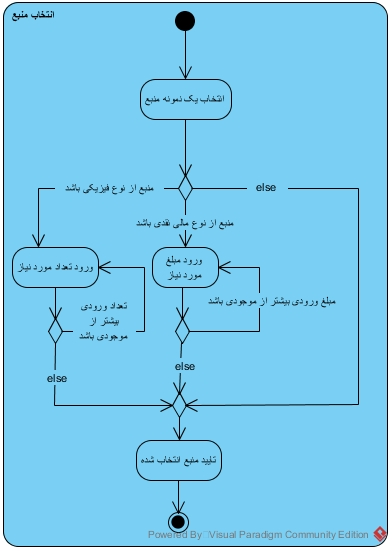
\includegraphics[scale=0.8]{img/activity/chooseres}
	\caption{انتخاب منبع}
\end{figure}


\section{تخصیص منبع به پروژه}
\begin{figure}[H]
	\centering
	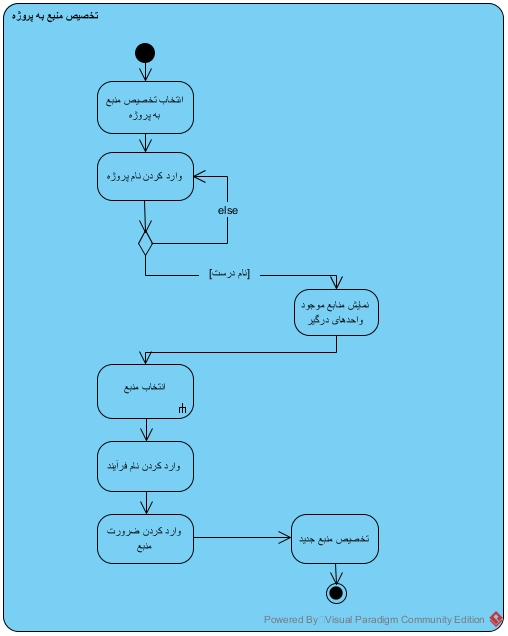
\includegraphics[scale=0.8]{img/activity/assres}
	\caption{تخصیص منبع به پروژه}
\end{figure}

\section{تعیین سطح دسترسی کاربر دیگر}
\begin{figure}[H]
	\centering
	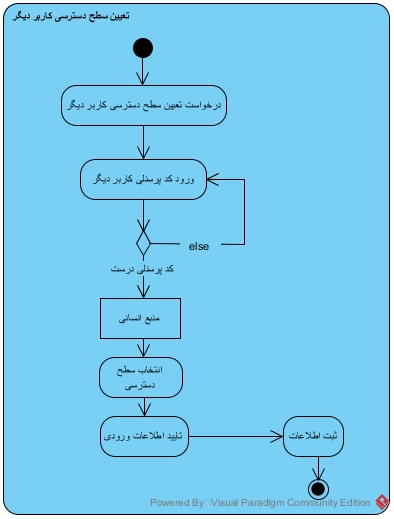
\includegraphics[scale=0.8]{img/activity/chooseacc}
	\caption{تعیین سطح دسترسی کاربر دیگر}
\end{figure}


\section{تعیین عملیات مجاز یک سطح دسترسی}
\begin{figure}[H]
	\centering
	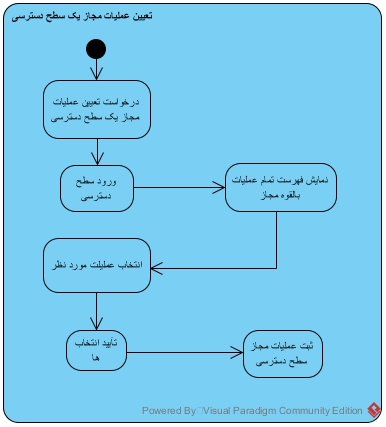
\includegraphics[scale=0.8]{img/activity/chooselev}
	\caption{تعیین عملیات مجاز یک سطح دسترسی}
\end{figure}


\section{تغییر سطح دسترسی کاربر دیگر}
\begin{figure}[H]
	\centering
	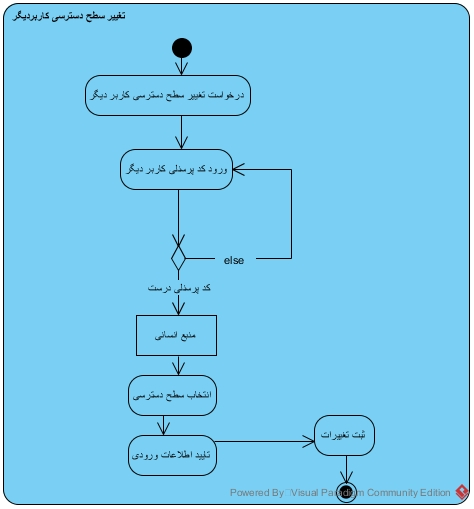
\includegraphics[scale=0.8]{img/activity/changeacc}
	\caption{تغییر سطح دسترسی کاربر دیگر}
\end{figure}


\section{تغییر مشخصات یک منبع}
\begin{figure}[H]
	\centering
	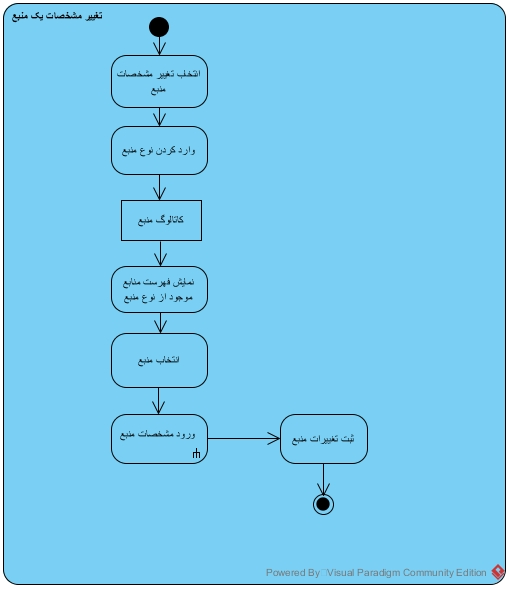
\includegraphics[scale=0.8]{img/activity/changeres}
	\caption{تغییر مشخصات یک منبع}
\end{figure}


\section{تهیه نسخه پشتیبان سیستم برنامه ریزی}
\begin{figure}[H]
	\centering
	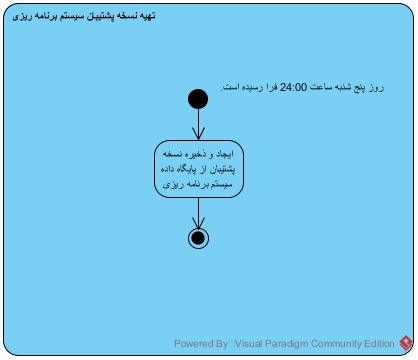
\includegraphics[scale=0.8]{img/activity/backup}
	\caption{تهیه نسخه پشتیبان سیستم برنامه ریزی}
\end{figure}

\section{ثبت تعداد استفاده کنندگان پروژه نرم افزاری}
\begin{figure}[H]
	\centering
	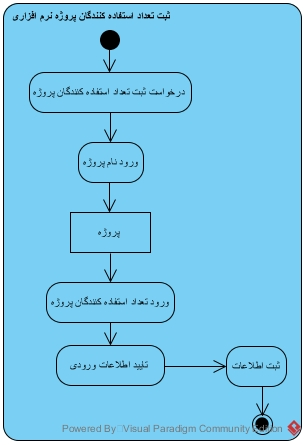
\includegraphics[scale=0.8]{img/activity/numusers}
	\caption{ثبت تعداد استفاده کنندگان پروژه نرم افزاری}
\end{figure}


\section{ثبت تغییر ماژول یک سیستم}
\begin{figure}[H]
	\centering
	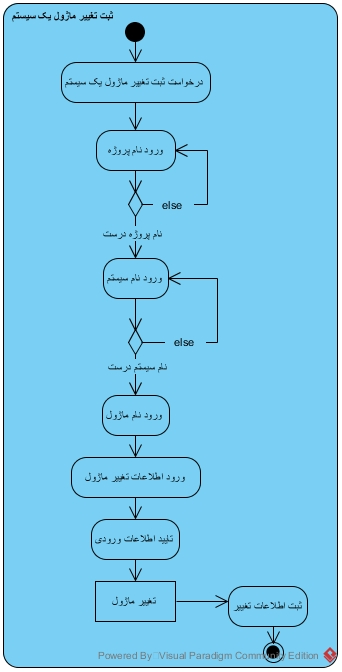
\includegraphics[scale=0.8]{img/activity/submod}
	\caption{ثبت تغییر ماژول یک سیستم}
\end{figure}


\section{ثبت تکنولوژی مورد استفاده پروژه نرم افزاری}
\begin{figure}[H]
	\centering
	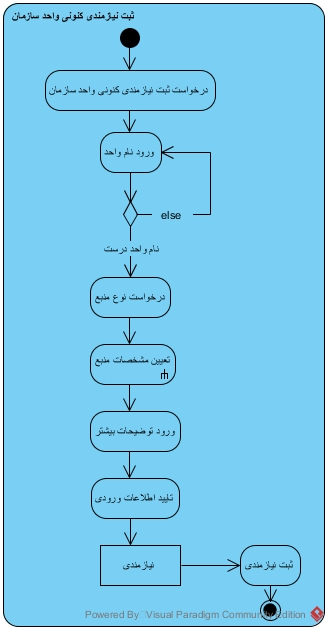
\includegraphics[scale=0.8]{img/activity/subreq}
	\caption{ثبت تکنولوژی مورد استفاده پروژه نرم افزاری}
\end{figure}

\section{ثبت نام در سیستم برنامه ریزی}
\begin{figure}[H]
	\centering
	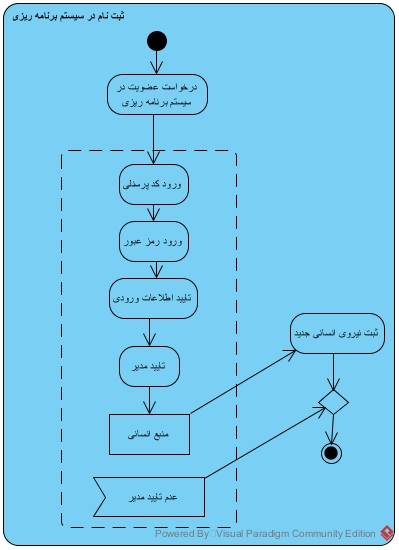
\includegraphics[scale=0.8]{img/activity/reg}
	\caption{ثبت نام در سیستم برنامه ریزی}
\end{figure}

\section{ثبت نیازمندی کنونی واحد سازمان}
\begin{figure}[H]
	\centering
	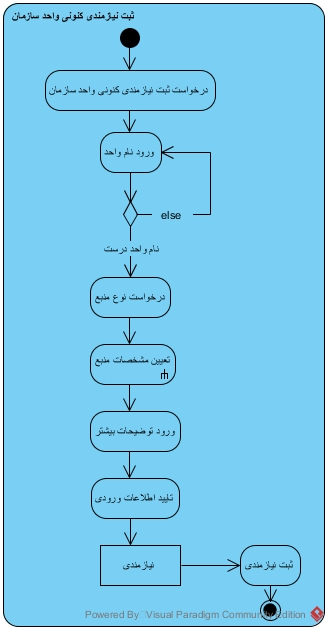
\includegraphics[scale=0.8]{img/activity/subreq}
	\caption{ثبت نیازمندی کنونی واحد سازمان}
\end{figure}

\section{جستجو در پروژه ها برای تخمین منبع}
\begin{figure}[H]
	\centering
	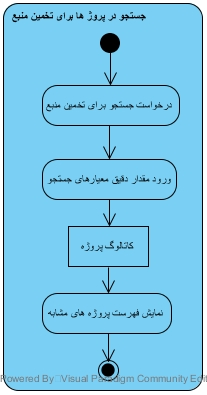
\includegraphics[scale=1]{img/activity/estres}
	\caption{جستجو در پروژه ها برای تخمین منبع}
\end{figure}

\section{جستجو در پروژه ها برای یافتن نیازمندی های ضروری}
\begin{figure}[H]
	\centering
	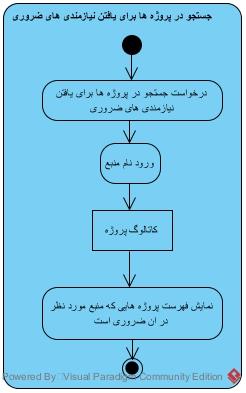
\includegraphics[scale=1]{img/activity/findessen}
	\caption{جستجو در پروژه ها برای یافتن نیازمندی های ضروری}
\end{figure}


\section{خروج از سیستم}
\begin{figure}[H]
	\centering
	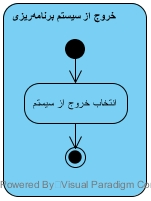
\includegraphics[scale=1]{img/activity/logout}
	\caption{خروج از سیستم}
\end{figure}


\section{دریافت گزارش جریان چرخشی مصرف منابع موجود}
\begin{figure}[H]
	\centering
	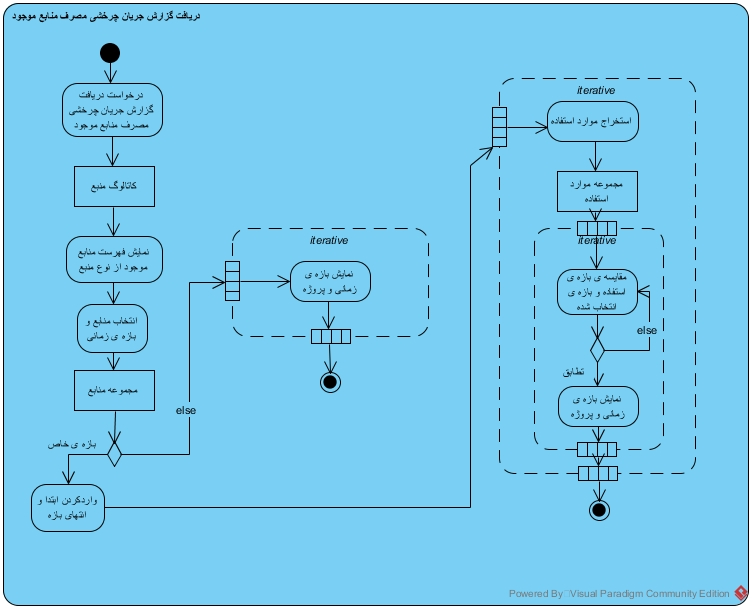
\includegraphics[scale=0.6]{img/activity/repflow}
	\caption{دریافت گزارش جریان چرخشی مصرف منابع موجود}
\end{figure}

\section{دریافت گزارش منابع موجود}
\begin{figure}[H]
	\centering
	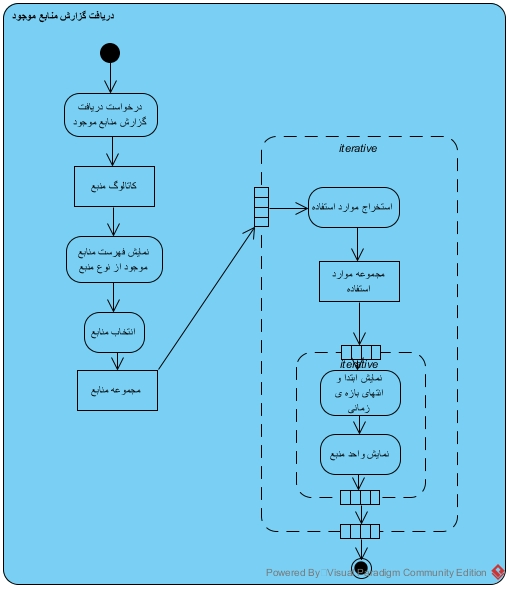
\includegraphics[scale=0.8]{img/activity/repavail}
	\caption{دریافت گزارش منابع موجود}
\end{figure}


\section{دریافت گزارش منابع مورد نیاز}
\begin{figure}[H]
	\centering
	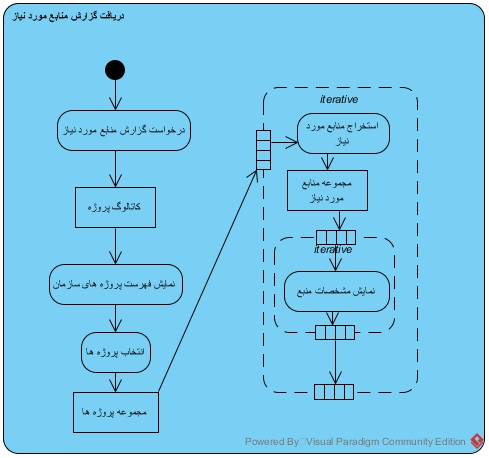
\includegraphics[scale=0.8]{img/activity/repneeded}
	\caption{دریافت گزارش منابع مورد نیاز}
\end{figure}

\section{مشاهده پروژه}
\begin{figure}[H]
	\centering
	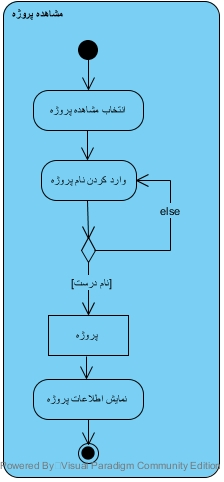
\includegraphics[scale=0.8]{img/activity/viewprj}
	\caption{مشاهده پروژه}
\end{figure}


\section{مشاهده فهرست پروژه‌ها}
\begin{figure}[H]
	\centering
	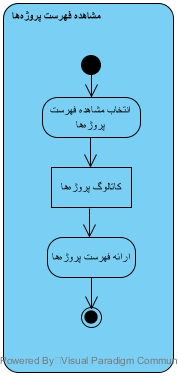
\includegraphics[scale=0.8]{img/activity/viewprjs}
	\caption{مشاهده فهرست پروژه‌ها}
\end{figure}


\section{مشاهده فهرست منابع یک واحد}
\begin{figure}[H]
	\centering
	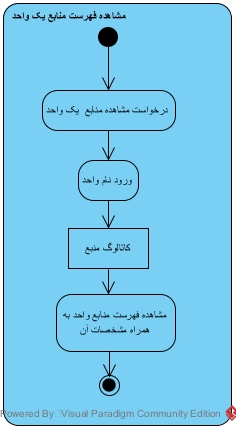
\includegraphics[scale=0.8]{img/activity/viewresunit}
	\caption{مشاهده فهرست منابع یک واحد}
\end{figure}

\section{مشاهده فهرست نیازمندی های یک واحد}
\begin{figure}[H]
	\centering
	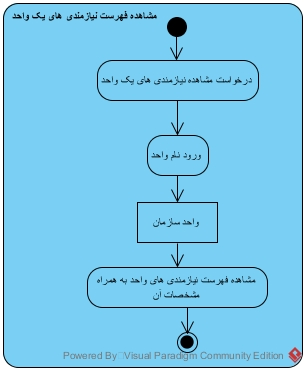
\includegraphics[scale=0.8]{img/activity/viewrequnit}
	\caption{مشاهده فهرست نیازمندی های یک واحد}
\end{figure}


\section{مشاهده مشخصات یک منبع}
\begin{figure}[H]
	\centering
	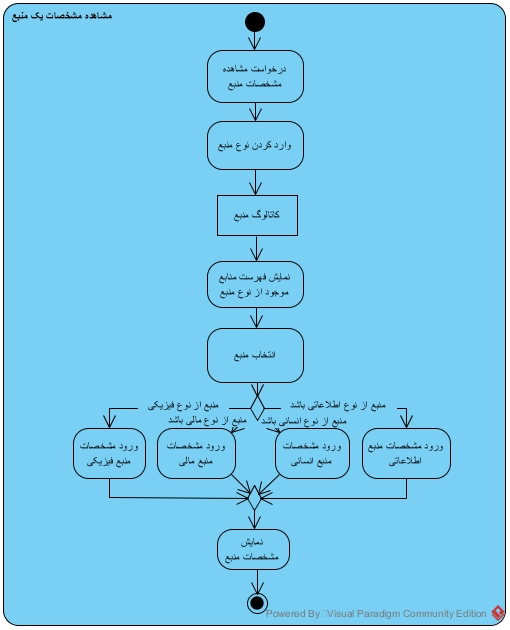
\includegraphics[scale=0.8]{img/activity/viewres}
	\caption{مشاهده مشخصات یک منبع}
\end{figure}

\section{ورود به سیستم}
\begin{figure}[H]
	\centering
	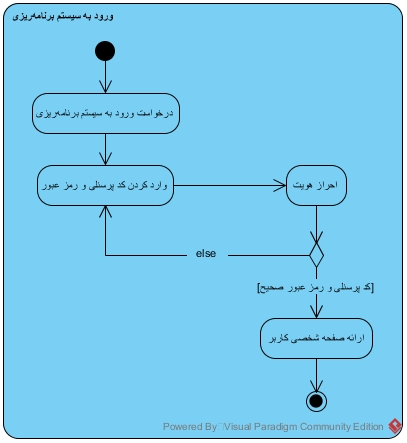
\includegraphics[scale=0.8]{img/activity/login}
	\caption{ورود به سیستم}
\end{figure}


\section{ورود مشخصات منبع}
\begin{figure}[H]
	\centering
	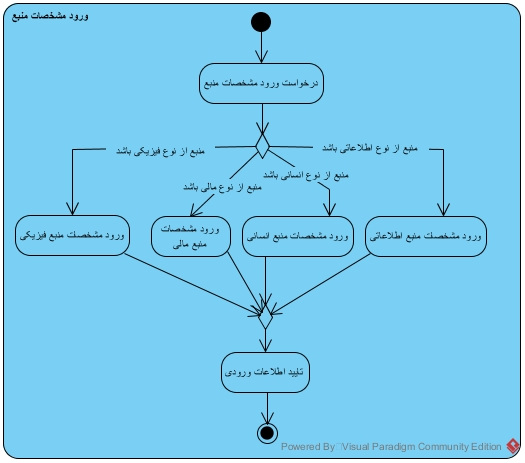
\includegraphics[scale=0.8]{img/activity/inputresprop}
	\caption{ورود مشخصات منبع}
\end{figure}